\documentclass{article}
\thispagestyle{empty}
\usepackage{tikz}
% plotting
\usepackage{pgf,tikz,pgfplots}
\usepackage{mathrsfs}
\usetikzlibrary{arrows}

\usepackage{tikz-cd} 
\usepackage{xcolor}
\usepackage{svg}



\begin{document}
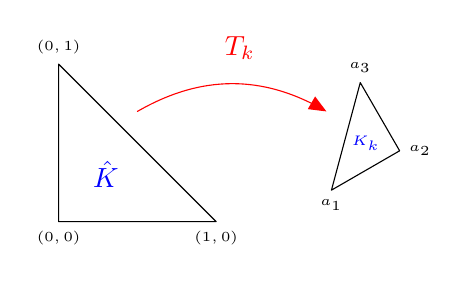
\begin{tikzpicture}[line cap=round,line join=round,>=triangle 45,x=2cm,y=2cm]
\draw (0,0) node[anchor=north]{\tiny $(0,0)$}
  -- (1,0) node[anchor=north]{\tiny $(1,0)$}
  -- (0,1) node[anchor=south]{\tiny $(0,1)$}
  -- cycle;
  
\node [color=blue] at (0.3,0.3) {$\hat{K}$};
  
  
\draw (1.73205081,0.2) node[anchor=north]{\tiny $a_1$}
  -- (2.16506351, 0.45) node[anchor=west]{\tiny $a_2$}
  -- (1.91506351, 0.8830127) node[anchor=south]{\tiny $a_3$}
  -- cycle;
  
 \node [color=blue] at (1.95,0.5) {\tiny $K_k$};
  
\draw [->,red] (0.5,0.7) to [bend left] (1.7,0.7);
 \node [color=red] at (1.15,1.1) {$T_k$};
\end{tikzpicture}
\end{document}
